\chapter{Fabrication Details}
\label{chap:fabrication}
\chaptermark{Fabrication Details}

This appendix describes, in detail, each of the steps taken to create the carbon nanotube (nanotube) devices measured for this thesis. Some of the information is specific to the Markovic lab and Johns Hopkins University, but an effort has been made to make the discussion useful to anyone producing nanotube devices.

The devices measured in this thesis were all produced with the following recipe:

\begin{enumerate}
\item Use the mask aligner (\ref{subsubsec:mask_aligner}) to pattern large sputtered molybdenum (\ref{subsec:sputtering}) leads on a silicon substrate
\item Pattern small catalyst islands (\ref{subsec:catalyst_island}) using electron beam lithography (\ref{sec:ebeam_lith})
\item Grow nanotubes directly on substrate using chemical vapor deposition (\ref{subsubsec:substrate_cvd})
\item Locate nanotubes using a scanning electron microscope (\ref{subsubsec:imaging_island})
\item Design devices using vector graphics software (\ref{sec:device_design})
\item Pattern devices using electron beam lithography (\ref{sec:ebeam_lith}) and thin film deposition (\ref{sec:thin_film})
\item Test device connectivity in the DC probe station (\ref{subsec:probe_station})
\item Wire bond connected devices in a chip carrier for further testing (\ref{subsec:wire_bonding})
\end{enumerate}

For details on each of the steps see the sections referenced. The rest of this appendix discusses additional methods and contains some useful observations made over several years spent producing nanotube devices.

\section{Wafer Preparation}

Each nanotube device began with a highly doped silicon substrate capped with an insulating layer. The wafers used were chosen for their low temperature electrical properties and ease of use.

\subsection{Selection and Cleaning}

All of the devices discussed in this thesis were built on highly n-doped silicon wafers with \ce{SiO2} capping layers. The wafers were purchased from Silicon Quest International. As ordered the wafers are 3 inches in diameter with a <100> silicon face. This crystal alignment allowed the wafers to be easily cleaved along the crystal axes using only a diamond scribe. The wafers are heavily n-doped with phosphorus giving them a resistivity of 10-\SI{20}{\ohm\centi\meter} down to the milliKelvin range. The oxide layers were \SI{300}{\angstrom} of thermally grown \ce{SiO2} and remained insulating at all measured temperatures.

Typically, wafers were cleaned by sonicating in acetone for 5 minutes, followed by an isopropanol rinse for 1 minute, and baking on a hot plate at about \SI{180}{\degreeCelsius} for 1 minute. This procedure was usually enough to ready the surface for lithography. In cases where cleanliness had to be improved, piranha etch was used to clean the wafers. 

Pirana etch is a mixture of 3:1 30\% sulfuric acid to 30\% hydrogen peroxide. It is important to be extremely careful with this wet etch as the solution is strongly exothermic. The wafers should be placed in the sulfuric acid, then the hydrogen peroxide is added slowly while stirring continuously. The solution will reach nearly \SI{200}{\degreeCelsius} within the first few minutes. After about 20 minutes, the solution should cool enough for the wafers to be removed. Surfaces cleaned in this way are free of organic and most metallic contaminates.

\subsection{Optical Lithography}
\label{subsec:optical}

The first step in building the devices discussed in this thesis was to pattern the substrate using optical lithography. In this process the wafer is first coated in a UV sensitive polymer resist. The wafer is then partially exposed to UV light and developed, leaving a patterned polymer mask through which thin films can be deposited.

The resists used can be either positive or negative tone. For this work, MicroChem S1813 was used as a positive tone resist and Futurex NR9 was the negative tone resist. Exposure, baking, and development times were chosen according to the manufacturer's instructions.

\subsubsection{Projection Lithography}
\label{subsubsec:project_lith}

Many of the devices produced in the Markovic lab have been patterned using the custom built projection lithography setup seen in Figure \ref{fig:project_lith}. The setup was built around a Nikon optical microscope. The microscope has been fitted with a UV lamp, movable UV filtering, and a custom mask holder.

\begin{figure}
    \centering
    \includegraphics[width = 1.0\textwidth]{appa/project_lith.eps}
    \caption{Custom projection lithography setup in the JHU physics department cleanroom. (a) The arrows from left to right show the UV lamp, sliding UV filter, and mask holder. (b) A projection lithography mask and holder. The arrow shows the mask itself.}
    \label{fig:project_lith}
\end{figure}

The masks were made using either a standard ink-jet printer or by a local printing company for higher resolution. The sample is placed under the desired objective, which determines the size of the pattern projected onto the sample. The mask is then inserted into the holder and then focused and positioned using the micrometer drives. Exposure times are  controlled by removing the UV filter from the light path. 

This setup is useful for quickly producing a few samples at a time. Specifically, it is used for producing graphene and nanowire devices, which require careful positioning of the pattern over the nanostructure of interest. The resolution limit of this technique is about \SI{2}{\micro\meter}. 

\subsubsection{Mask Aligner}
\label{subsubsec:mask_aligner}

For production of many, identical devices, projection lithography as described in Section \ref{subsubsec:project_lith} becomes extremely tedious. This problem was solved by use of a mask aligner. 

\begin{figure}
    \centering
    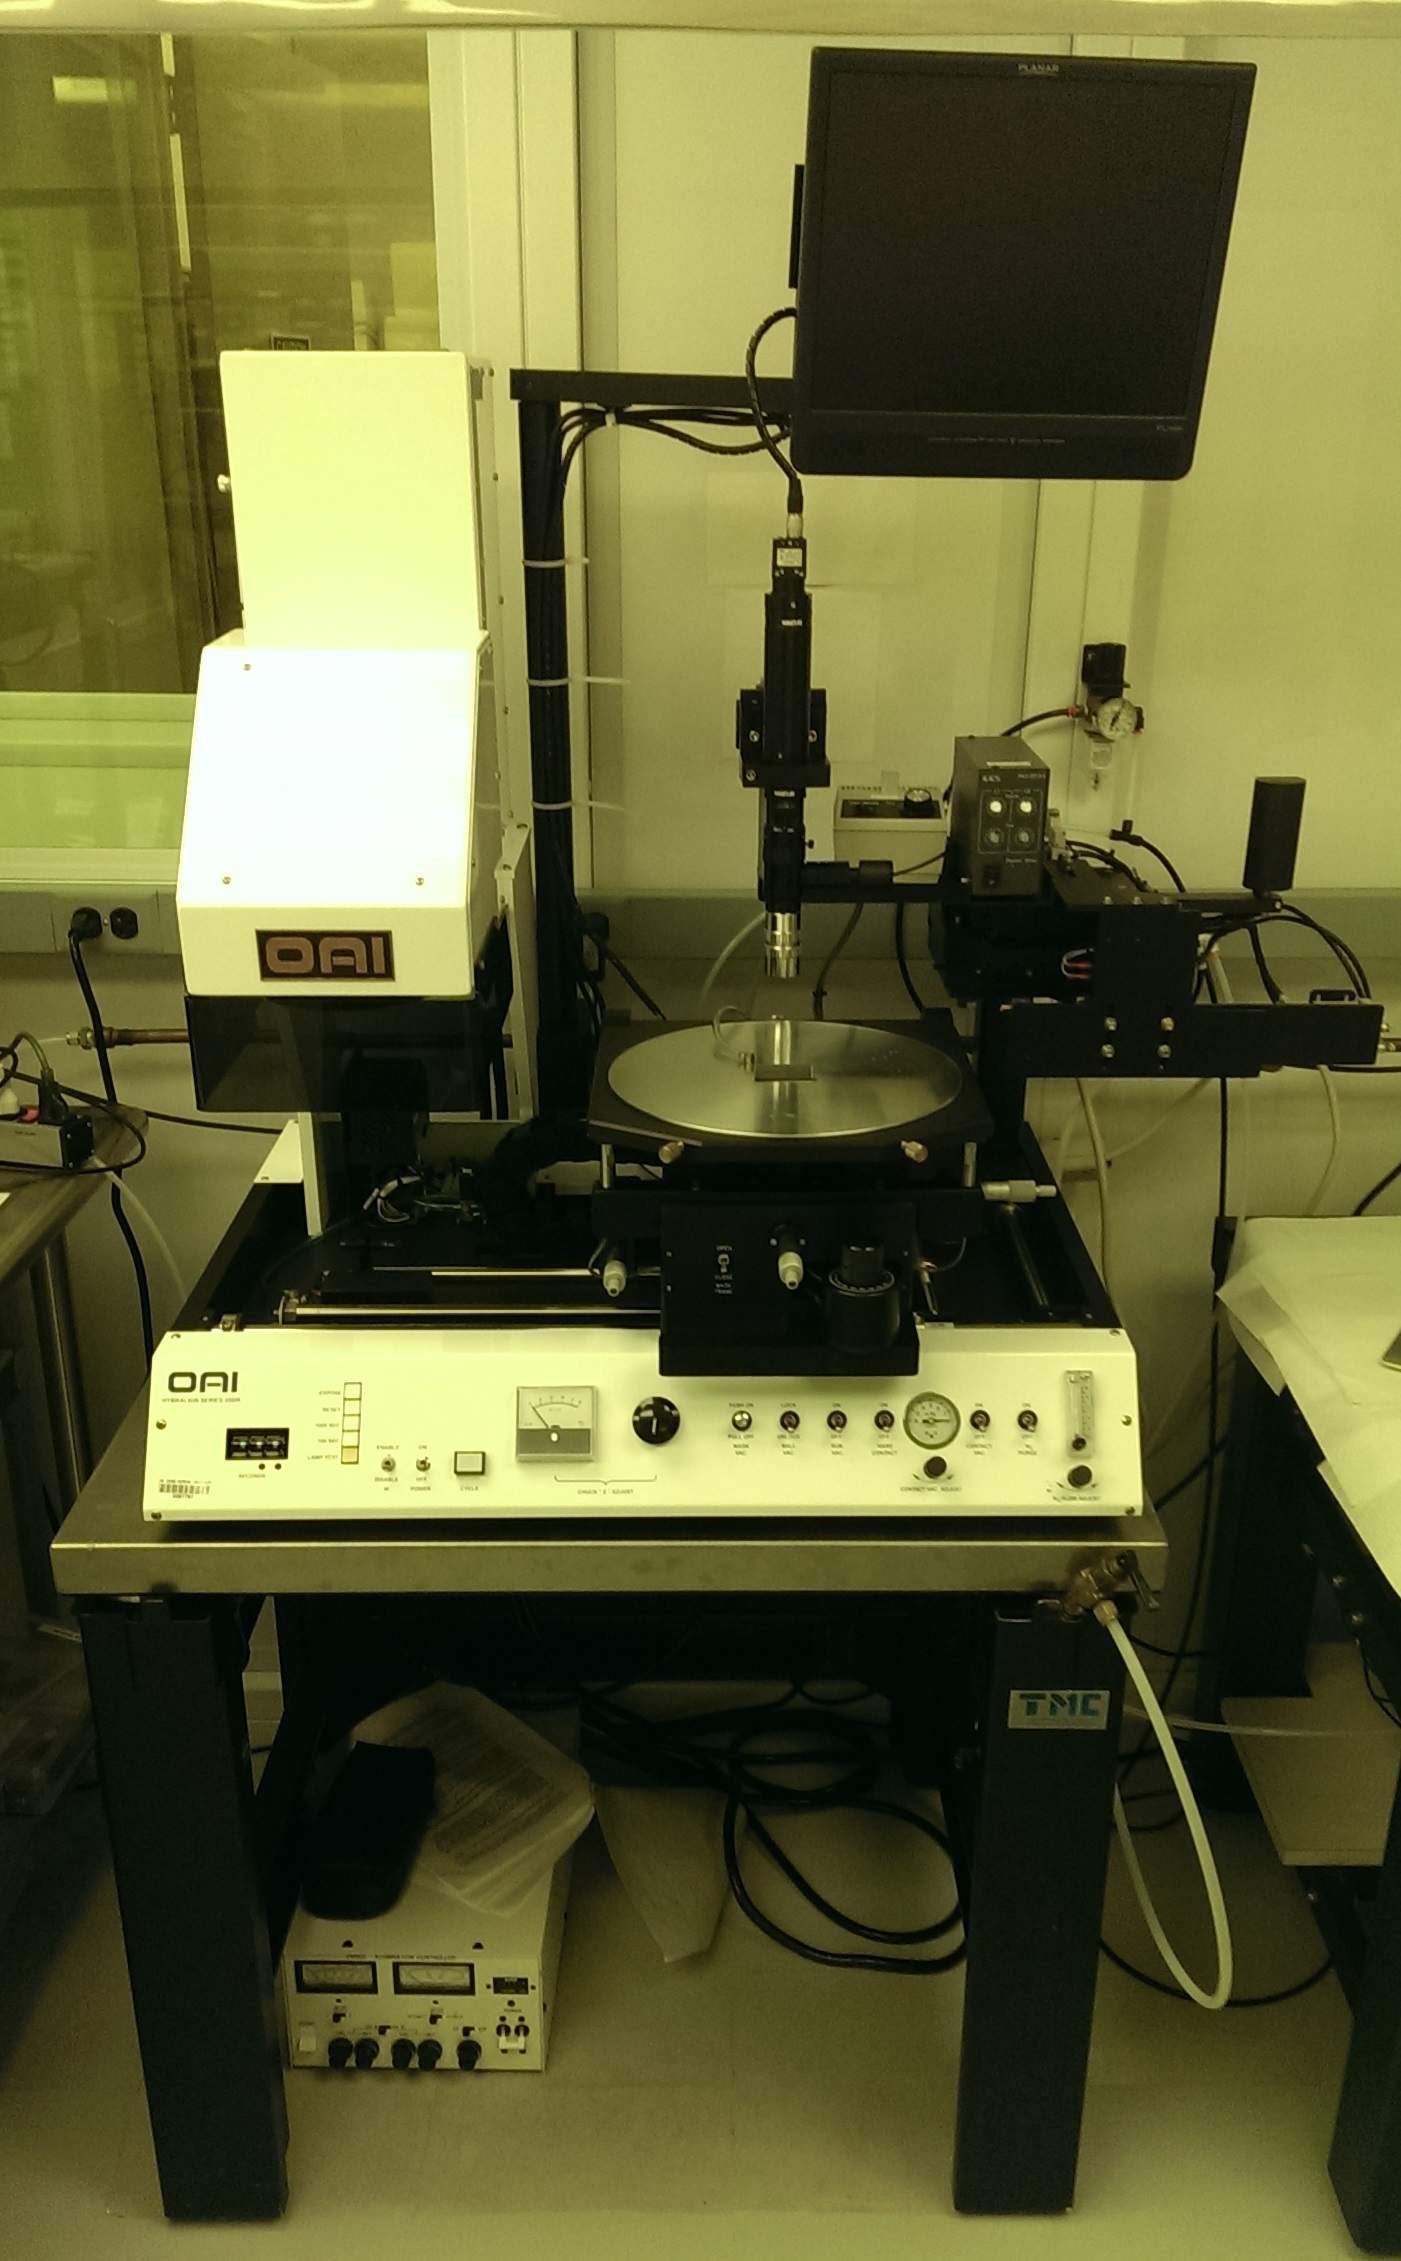
\includegraphics[width = 1.0\textwidth]{appa/mask_aligner.eps}
    \caption{OAI mask aligner in the JHU physics department cleanroom. (a) The mask aligner. (b) A typical 3" chromium on glass mask.}
    \label{fig:mask_aligner}
\end{figure}

First, a chromium on glass mask is made with the desired pattern in the actual size, as seen in Figure \ref{fig:mask_aligner}. The mask is then loaded into the aligner and a substrate, coated with polymer resist, is mounted under it. Finally, the mask and substrate are pressed together and exposed to a UV light source. The resolution of the OAI mask aligner is about \SI{1}{\micro\meter}.

\section{Device Design}
\label{sec:device_design}

Once the substrates are prepared, devices are designed one at a time using Adobe Illustrator. Any computer aided drafting (CAD) or vector graphics program would work just as well. The procedure is outlined in Figure \ref{fig:device_design}. Designing the devices is a simple process of connecting the nanotubes with the mask aligner leads, although some thought must be given to the size of the leads drawn. If the leads are too large, the write time for the electron beam lithography steps will be too long. Additionally, one must be careful not to let any stray nanotubes short the device leads.

\begin{figure}
	\centering
	\includegraphics[width = 1.0\textwidth]{appa/device_design.eps}
	\caption{Adobe Illustrator designs used for optical and electron beam lithography masks. (a) The pink outlines show the large molybdenum leads patterned with the mask aligner. Inside that pattern are the four \SI{3}{\micro\meter} catalyst islands patterned with electron beam lithography. (b) An SEM micrograph of a sample after CVD growth fitted into the pattern. (c) A complete circuit design. In this case, the layers are normal metal (green), ferromagnet (purple), and superconductor (blue).} 
	\label{fig:device_design}
\end{figure}

\section{Electron Beam Lithography}
\label{sec:ebeam_lith}

Electron beam lithography is the process of creating masks by patterning a polymer resist by exposure to a focused beam of electrons. In the Johns Hopkins physics department the electron beam lithography setup is based around a Zeiss EVO50 scanning electron microscope. The microscope is controlled by Zeiss SmartSEM software. Attached to the microscope control computer by a serial port is a second computer running Elphy Quantum, electron beam lithography software from Raith. The Raith software can take control of the beam to write patterns based on GDSII drawings. The SEM setup is shown in Figure \ref{fig:sem_setup}.

\begin{figure}
	\centering
	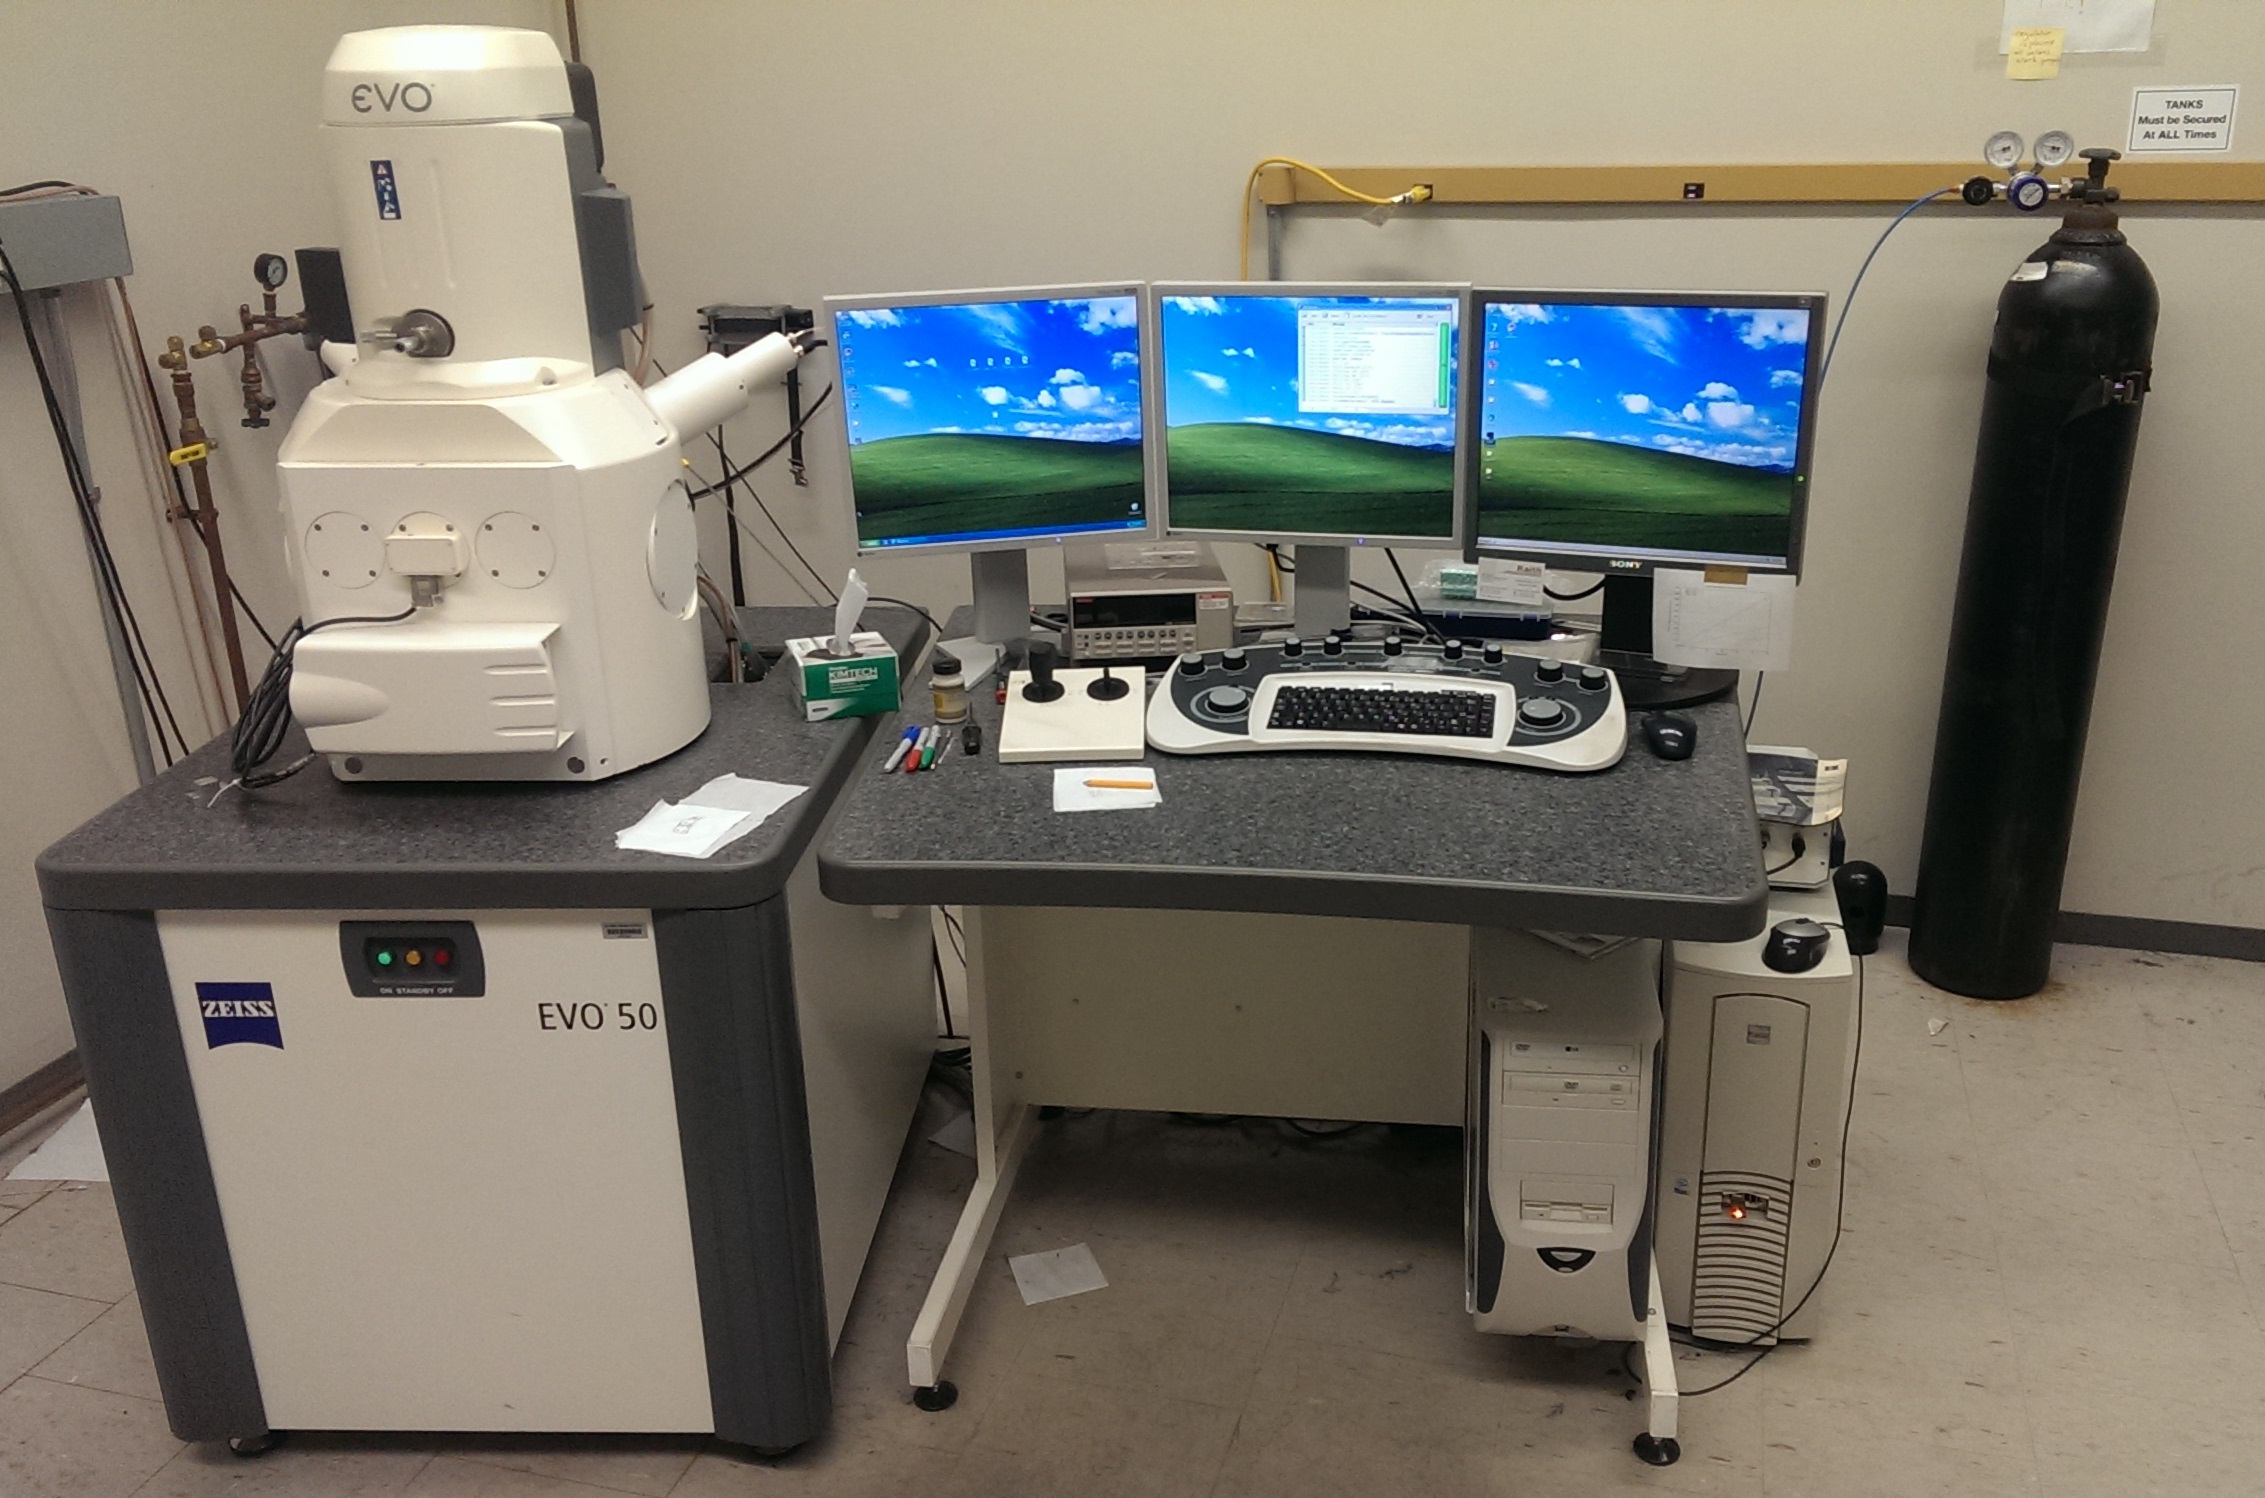
\includegraphics[width = 0.8\textwidth]{appa/sem_setup.jpg}
	\caption{Zeiss EVO50 SEM with Raith control computer and external beam blanker.}
	\label{fig:sem_setup}
\end{figure}

The electron beam sensitive resist used in all of this work was polymethyl methacrylate (PMMA) from MicroChem. PMMA is a polymer that, after baking on a hot plate, forms copolymer bonds that can be broken by exposure to a beam of electrons. Once these bonds are broken, the unbonded polymer can be washed away by a developer, leaving trenches in the PMMA wherever it was exposed to the electron beam. The patterned mask can later be removed by soaking in acetone.

\subsection{Standard Recipe}

\begin{table}
	\centering
	\caption{Standard PMMA/MIBK recipe}
	%\hfill \\
    \begin{tabular}{ r | l }
    	\hline
    	EHT Voltage & \SI{30}{\kilo\electronvolt} \\ \hline
    	Beam Current & \SI{40}{\pico\ampere} \\ \hline
    	Step Size & \SI{10}{\nano\meter} \\ \hline
    	Dose & \SI{300}{\micro\coulomb\per\square\centi\meter} \\ \hline
    	Developer & 1:3 MIBK:IPA \\ \hline
    	Development time & 60s \\ \hline
    	Post-development & rinse 30s in IPA \\ \hline
    \end{tabular}
    \label{table:standard_pmma}
\end{table}

This recipe, using room temperature methyl isobutyl ketone (MIBK) as a PMMA developer, is the simplest recipe to start with for almost any project requiring electron beam lithography. The relevant parameters are shown in Table \ref{table:standard_pmma}.

\subsection{Cold Development}

\begin{table}
	\centering
	\caption{Cold developer recipe}
	%\hfill \\
    \begin{tabular}{ r | l }
    	\hline
    	EHT Voltage & \SI{30}{\kilo\electronvolt} \\ \hline
    	Beam Current & \SI{40}{\pico\ampere} \\ \hline
    	Step Size & \SI{10}{\nano\meter} \\ \hline
    	Dose & \SI{1400}{\micro\coulomb\per\square\centi\meter} \\ \hline
    	Developer & 7:3 IPA:water at \SI{0}{\degreeCelsius} \\ \hline
    	Development time & 90s \\ \hline
    	Post-development & rinse 30s in water \\ \hline
    \end{tabular}
    \label{table:cold_pmma}
\end{table}

It was discovered in 2004, that by lowering the development temperature and increasing the dose, the resolution of PMMA could be improved significantly \cite{Hu2004}. This has been shown using MIBK:IPA as a developer as well as various mixtures of IPA and water \cite{Cord2007, Yasin2002, Rooks2002, Koshelev2011}. The best results obtained in our lab were using IPA and water. The recipe is shown in Table \ref{table:cold_pmma}. The improved contrast can be attributed to the higher dose. By increasing the dose and decreasing the efficacy of the developer, the negative effects of backscattered electrons passing through the PMMA are diminished.

\section{Thin Film Deposition}
\label{sec:thin_film}

In this work, thin film deposition is used (along with polymer masks patterned with optical or electron beam lithography) to create circuits around carbon nanotubes. There are three main methods used; each method will be discussed along with a few materials typically deposited in that way. 

\subsection{Thermal Evaporation}
\label{subsec:thermal_evap}

Thermal evaporation is the simplest method of thin film deposition discussed here. The material to be evaporated is placed in a boat, typically made of tungsten, alumina, or both. Substrates for the film to be deposited on are located above the evaporation boat. Both the boat and the samples are placed in a high vacuum chamber. Once the chamber has reached around \SI{1d-7}{\torr}, current through the evaporation boat is increased until the material melts or begins to sublimate. The deposited thickness and deposition rate are monitored using a quartz crystal monitor. Once the desired rate is reached, a shutter is opened to expose the sample to the evaporated material. 

This type of evaporation is best used with materials that have a relatively low melting point ($\lesssim$\SI{1200}{\degreeCelsius}). Two evaporators were used in this work, a 1970s Denton evaporator fitted with a newer Hewlett Packard power supply, and an early 2000s Torr thermal evaporator. The Torr chamber is kept free from magnetic materials in hopes of limiting contamination of superconducting films. Some common materials and the boats we have found most useful are listed in Table \ref{table:thermal_evap}.

\begin{table}
	\centering
	\caption{Thermal evaporation materials}
	%\hfill \\
	\begin{tabular}{r | p{60mm}}
		\hline
		Au & alumina coated W crucible \\ \hline
		Ti & long, narrow W boat \\ \hline
		Cr & chrome plated W rod\\ \hline
		Al & dimpled W boat \\ \hline
		Co & alumina coated W crucible (does not last long) \\ \hline
	\end{tabular}
	\label{table:thermal_evap}
\end{table}	

\subsection{Electron Beam Evaporation}
\label{subsec:ebeam_evap}

Electron beam evaporation uses a high energy (\SI{7.5}{\kilo\electronvolt}) beam of electrons to melt the source material. The electron gun sits under a crucible full of the source material. The electron beam generated is bent and rastered across the center of the crucible using a strong magnetic field. Substrates are placed above the crucible and as the material melts and evaporates it is deposited on the substrate.

This method of evaporation has two benefits over thermal evaporation. First, it can be used for materials with a higher melting point. In the case of the Sharon Vacuum electron beam evaporator used in this work, materials with melting points up to $\sim$\SI{1800}{\degreeCelsius} were successfully evaporated. Second, the evaporated films are typically a little cleaner because the crucible, unlike thermal evaporation boats, does not have to be heated in order for the source material to melt. 

Due to limited access to the evaporator, not many of the films discussed in this work were deposited with electron beam evaporation. However, we have successfully deposited Nb, Co, Ti, and Al films all from graphite crucibles. Graphite was chosen here because of its affordability. There are likely better choices of crucible available. 

\subsection{Sputtering}
\label{subsec:sputtering}

Magnetron sputtering is a great method to deposit an amorphous thin film of just about any material needed. The three-target sputtering chamber used in this work was custom built by Professor Chia-Ling Chien's group at Johns Hopkins.

To sputter a material, a target 1-2 inches in diameter is loaded onto a cathode at the bottom of a vacuum chamber. The substrate to be coated is placed above the target on the anode. Once the system is at high vacuum,  argon gas (or any inert gas) is introduced to the chamber. An argon plasma is ignited between the cathode (target) and anode (sample). The strong electric potential and magnetic field from permanent magnets placed under the target focus the plasma in a ring pattern on the face of the target. Argon ions bombard the target and target atoms are ejected toward the substrate mounted above. 

The benefit of sputtering, as mentioned above, is that almost any metal can be sputtered with a DC plasma (RF plasma is used for insulating materials). Due to the high energy of the argon ions and ejected target atoms, this method can damage some sensitive samples. There may be some evidence that this is the case with carbon nanotube samples. For this work, low energy plasma was used to keep the average energy of ejected target atoms around a few eV. This is about 10 times higher than the energies used in thermal and electron beam evaporation. Even if sputtering does introduce some damage to nanotube samples, it does not appear to be the primary source of disorder.

\subsection{Atomic Layer Deposition}
\label{subsec:ald}

\begin{figure}
	\centering
	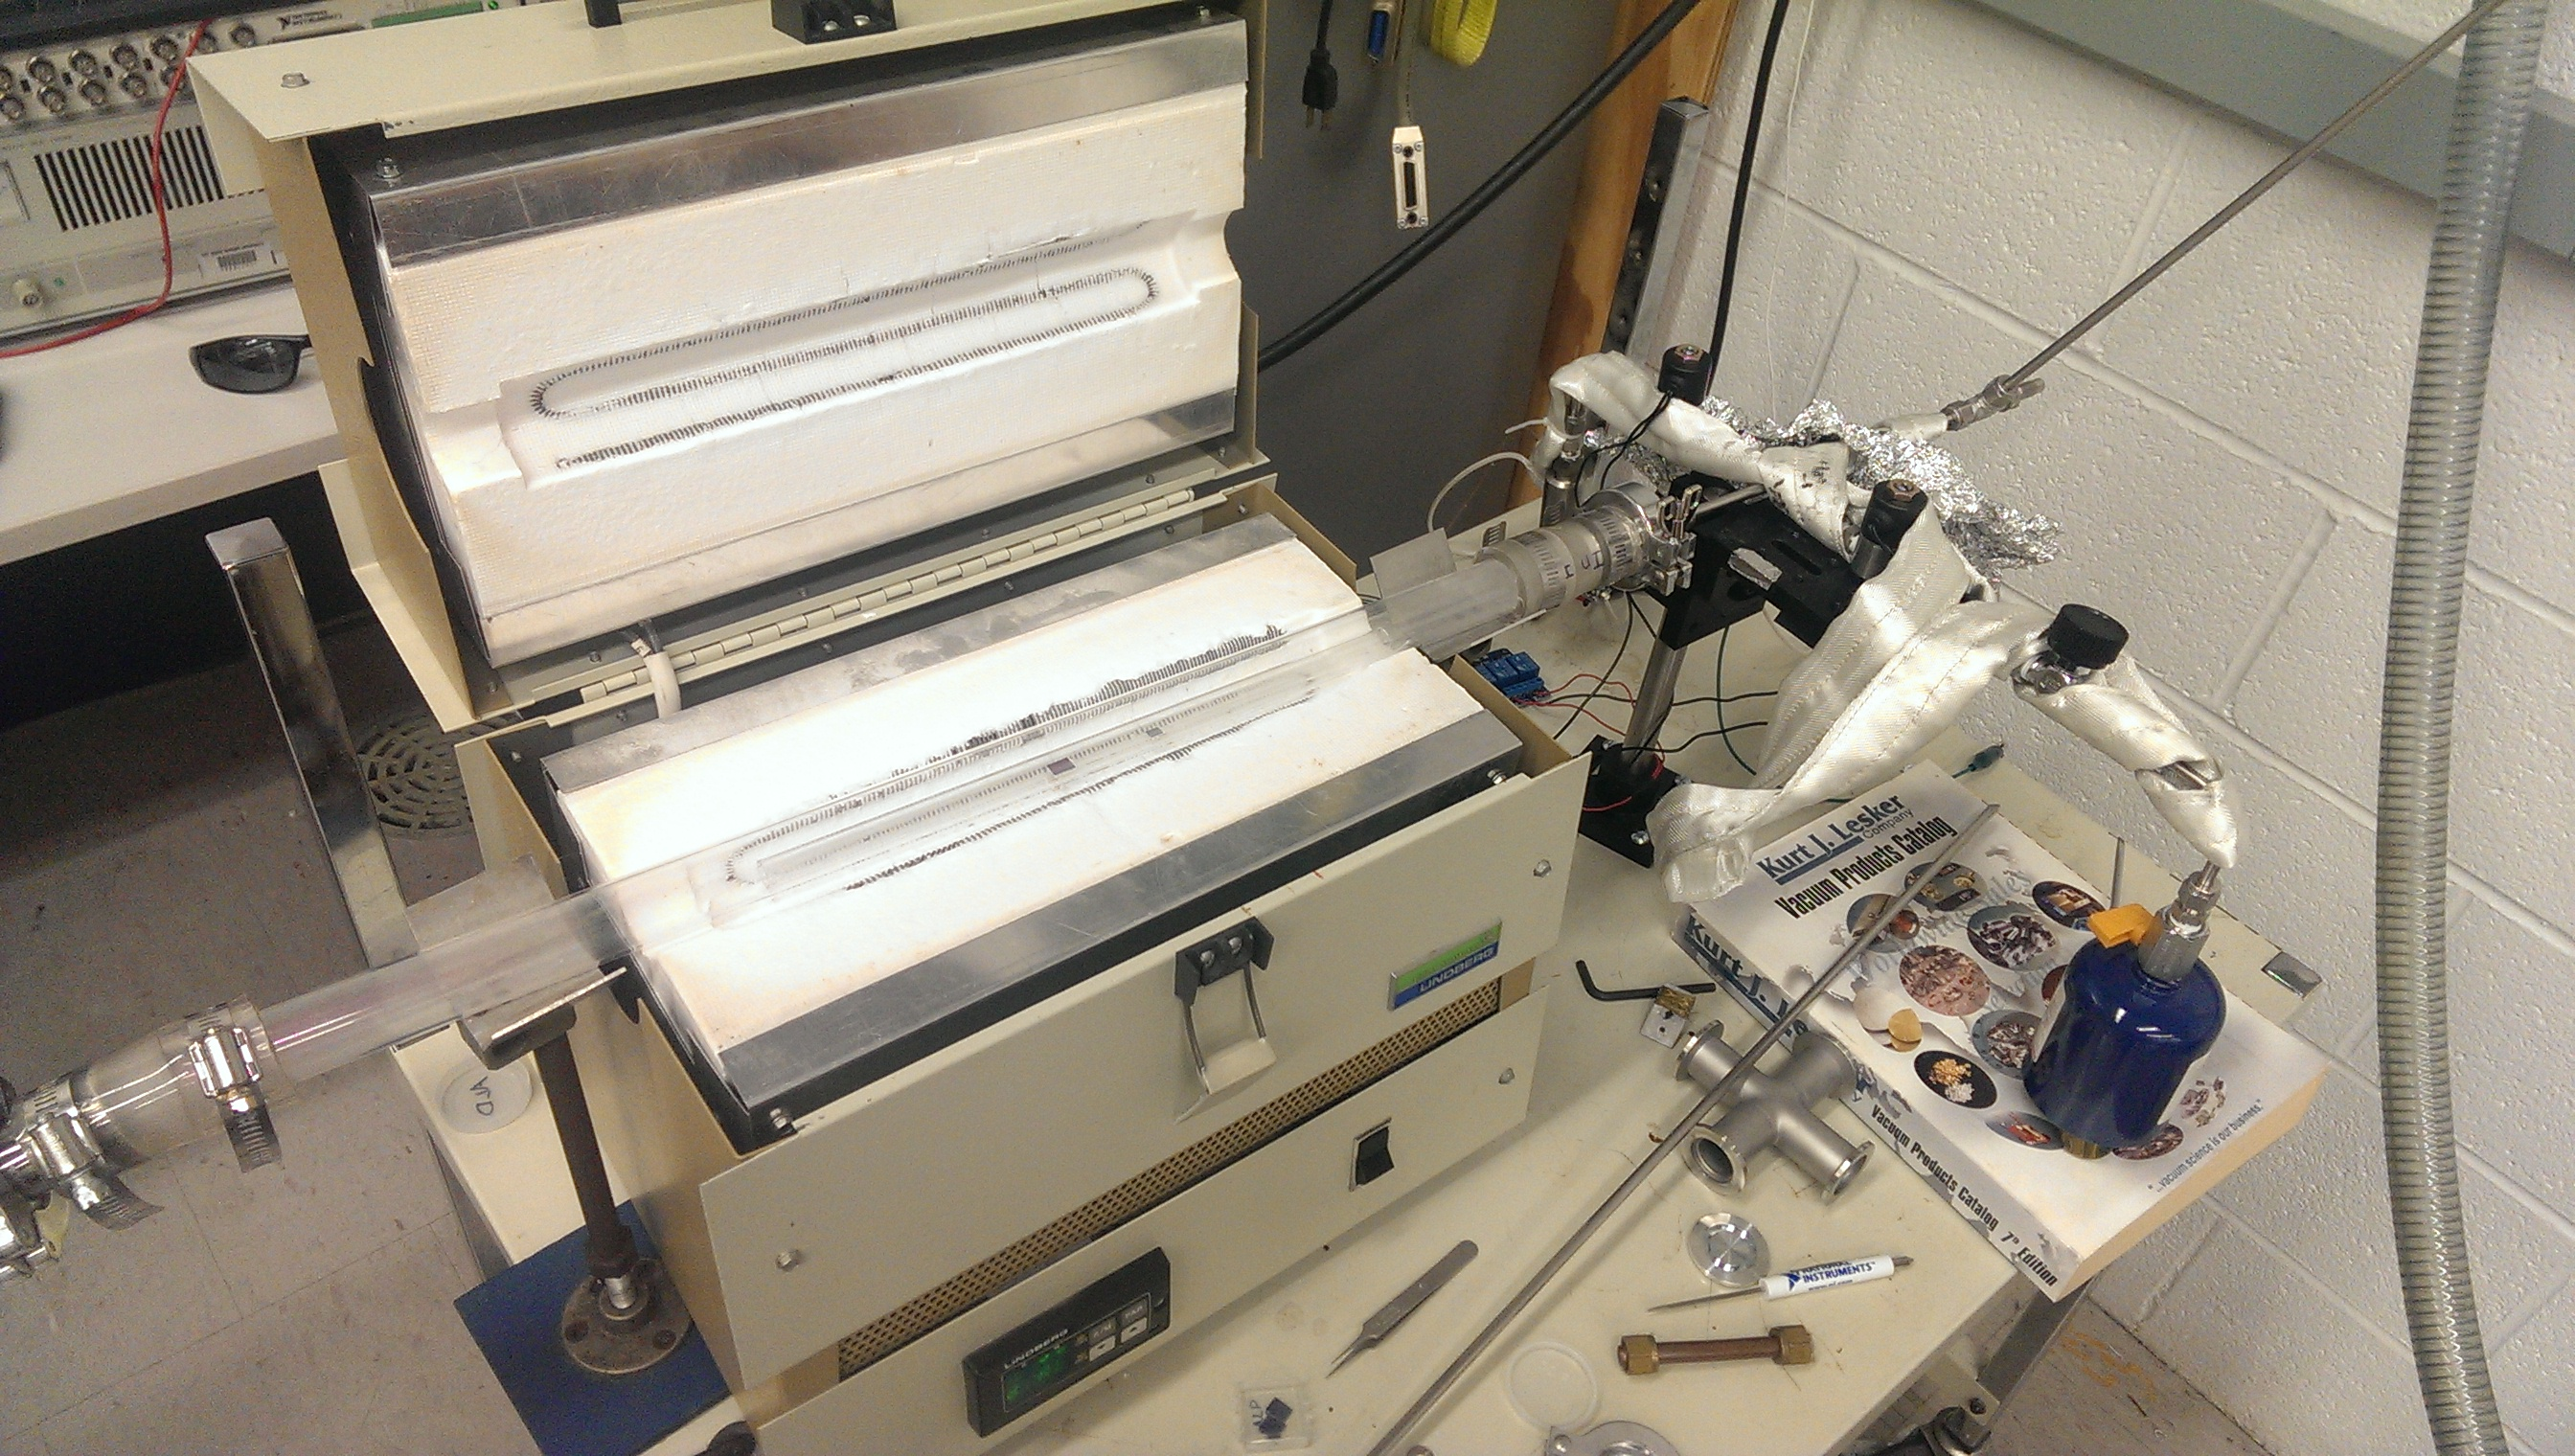
\includegraphics[width = 0.8\textwidth]{appa/ald.jpg}
	\caption{The Markovic lab ALD reactor. Gas flow is from right to left.} 
	\label{fig:ald}
\end{figure}

Atomic layer deposition (ALD) is a process in which thin, usually insulating, films are grown by reacting a series of gases. As a part of this work, we have constructed a homemade ALD reactor in the Markovic lab with the help of Streit Cunningham. It uses the same Lindberg 1 inch tube furnace as the chemical vapor deposition setup.

Samples are loaded into a 1 inch quartz tube and placed in the furnace. The tube is evacuated to about \SI{100}{\milli\torr} using a mechanical rough pump. A high purity \ce{N2} flow is turned on and adjusted so the pressure in the chamber, with the pump still running, is \SI{1000}{\milli\torr}. The \ce{N2} flow will act as a carrier gas throughout the process. We have only tested the reactor for growth of \ce{Al2O3} layers. Two precursor gases are used in the growth of \ce{Al2O3}, water vapor and trimethylaluminum (TMA). Once the quartz tube is evacuated and \ce{N2} flow is set, the water vapor and TMA are alternately pulsed using computer controlled solenoid valves. Films grow one monolayer (\SI{1.1}{\angstrom}) per pulse cycle. A typical recipe is as follows:

\begin{enumerate}
\item Evacuate tube to \SI{100}{\milli\torr} with mechanical pump
\item Turn on \ce{N2} flow such that the pressure reaches \SI{1000}{\milli\torr}
\item Set furnace temperature to \SI{130}{\degreeCelsius}
\item Pulse TMA for 1 second
\item Purge for 60 seconds
\item Pulse water for 1 second
\item Purge for 60 seconds
\item Repeat pulse\slash purge cycle until desired thickness has been reached
\item Cool furnace, turn off \ce{N2} flow, turn off pump, remove sample
\end{enumerate}

The goal with this recipe is to grow a quality insulating layer at a temperature low enough to be compatible with PMMA processing. This design is based on previous low temperature ALD growth by the George lab at the University of Colorado Boulder \cite{Elam2002, Groner2004}.

\subsection{Liftoff}
\label{subsec:liftoff}

When patterning a thin film using a polymer mask, such as PMMA or S1813, the final step after deposition of the film is to remove the mask. This process is called liftoff, as the excess metal is lifted off the substrate along with the dissolved polymer mask.

Typically, liftoff is very simple. The sample is soaked in acetone for 1-12 hours (depending on what else is going on in the lab), then rinsed in IPA for 30 seconds followed by a 30 second rinse in water. 

To help remove any stubborn material the sample can be sprayed with a bottle of acetone for a few seconds before rinsing in IPA. Some samples can also be placed in a beaker of acetone in a sonicator for a few seconds before rinsing in IPA. Sonication is not ideal for nanotube samples, as the process tends to break nanotubes off of the substrate and introduce defects in long tubes. An example of this can be seen in Figure \ref{fig:broken_tube}.

\begin{figure}
	\centering
	\includegraphics[width = 1.0\textwidth]{appa/broken_tube.eps}
	\caption{(a) A substrate with catalyst islands and a few long nanotubes before patterning. (b) The same substrate after patterning and liftoff. Comparing the two images, it is clear that the use of sonication during liftoff has broken many of the nanotubes.}
	\label{fig:broken_tube}
\end{figure}

\section{Room Temperature Testing}

After devices have been fabricated, it is important to check the connectivity of the devices before spending the time to load samples into a cryostat.

\subsection{Probe Station}
\label{subsec:probe_station}

The first step after fabrication is to test the resistance, and sometimes the gate behavior, of a device using a DC probe station. Our DC probe station was custom built for our lab and can be seen in Figure \ref{fig:probe_station}.

\begin{figure}
	\centering
	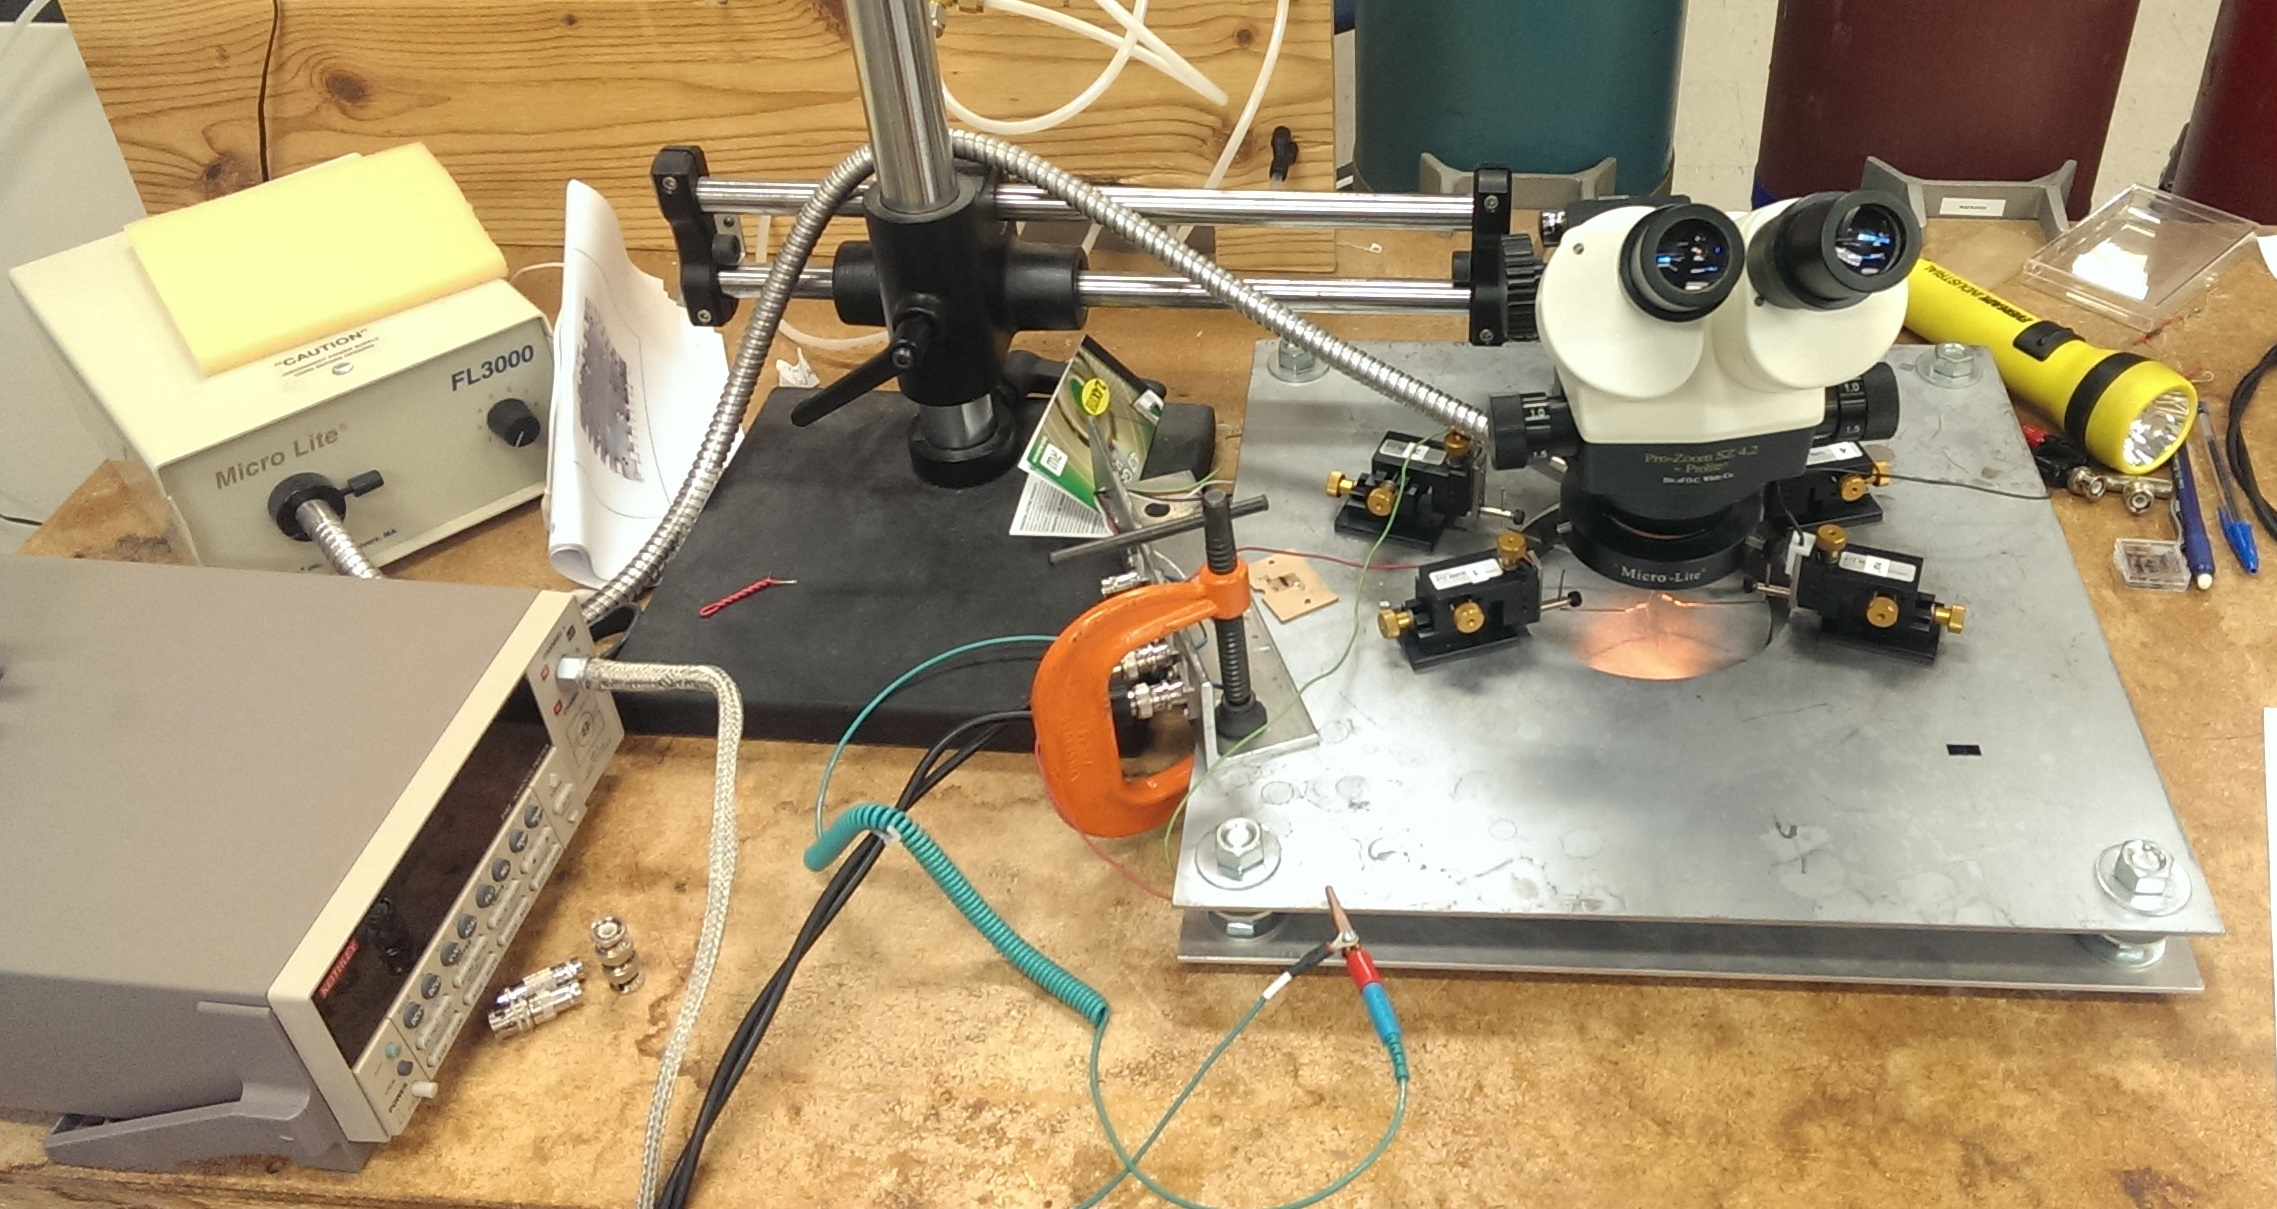
\includegraphics[width=0.8\textwidth]{appa/probe_station.jpg}
	\caption{The Markovic lab probe station. Four sharp probes are located under an optical microscope. Each can be connected to external sources and measurements using BNC connectors.}
	\label{fig:probe_station}
\end{figure}

The simplest and safest way found to check nanotube devices is to apply a small DC voltage (a few \si{\milli\volt}) between two of the large leads and measure the current with an ammeter. The measurements are done using a real-time LabView program. The bias is supplied by a National Instruments DAQ board through a $10^{-2}$ voltage divider. Current is measured by the same DAQ board by monitoring the output of an Ithaco 1211 current-to-voltage amplifier. 

\subsection{Wire Bonding}
\label{subsec:wire_bonding}

The final step in preparing devices for measurement is to wire bond the sample into a chip carrier. Each chip carrier is about \SI{1}{\centi\meter} square and fits into a standard socket on each of our cryostats. The wire bonder is used to connect the large optical lithography leads on the sample to the chip carrier. An old Kulicke and Soffa wire bonder in Chia-Ling Chien's lab was used for this work. It can be seen in Figure \ref{fig:wire_bonder}a.

\begin{figure}
	\centering
	\includegraphics[width=1.0\textwidth]{appa/wire_bonder.eps}
	\caption{(a) Kulicke and Soffa wire bonder. (b) An optical image of a completed device mounted in a chip carrier. (c) An SEM image detailing aluminum wires bonded to large gold leads.}
	\label{fig:wire_bonder}
\end{figure}

The wire bonder is used to connect a point on the chip carrier to a point on the sample with an aluminum or gold thread. The thread is first pressed by the wire bonder tip onto a bonding pad on the chip carrier. When the wire is in contact with the bonding pad the tip vibrates and presses down onto the sample to fix the wire into place. The tip can then be moved to contact one of the large optical lithography leads on the sample with the same wire. Once the second bond is made, the tip pulls away quickly to break the wire. The results of this process can be seen in Figures \ref{fig:wire_bonder}b and c.
